\documentclass[11pt]{beamer}
\usepackage[utf8]{inputenc}
\usepackage[T1]{fontenc}
\usepackage{lmodern}
\usepackage{listings}
\usetheme{Madrid}
\usepackage{hyperref}
\begin{document}
	\author{GROUPE 2}
	\title{M2 SLED 2023/2024}
	\subtitle{}
	%\logo{}
	\institute{}
	\date{\tiny Feb 29,  2024}
	\subject{}
	%\setbeamercovered{transparent}
	%\setbeamertemplate{navigation symbols}{}
	\begin{frame}[plain]
		\title{ {\small Problème du sac a dos avec Méthode de recherche locale itérée (Iterated local search)}}
		\author{{\tiny MASTER II SYTEMES ET LOGICIELS EN ENVIRONNEMENT DISTRIBUE(SLED)}\\ {\tiny Groupe 2}\\ {\tiny Examinateur: Pr. NDAM } }

		\begin{center}	
			{\footnotesize	UNIVERSITE DE NGAOUNDERE }	\\
		 {\tiny FACULTE DES SCIENCES }\\
		 {\tiny DEPARTEMENT DE MATHEMATIQUES ET INFORMATIQUE}\\
	 		
\includegraphics[scale=0.1]{image}\\
	 \end{center}
		\maketitle
		 
	\end{frame}
	
	\begin{frame}
		\frametitle{Plan du travail}
		\tableofcontents
	\end{frame}

% Section 1: Introduction
\section{Introduction}
\begin{frame}{Introduction}
   \begin{block}{Le Problème du Sac à Dos}
        Le problème du sac à dos est un problème classique d’optimisation combinatoire où l’objectif est de maximiser la valeur des objets placés dans un sac à dos tout en respectant sa capacité maximale. Il est largement étudié dans les domaines de l’informatique, de la logistique et de l’ingénierie pour ses nombreuses applications pratiques.
    \end{block}
    
    
        Dans cet exposé, nous aborderons une approche spécifique pour résoudre ce problème : la méthode de recherche locale itérée.
    
  
\end{frame}

% Section 2: Méthode de Recherche Locale Itérée
\section{Méthode de Recherche Locale Itérée}
\begin{frame}{Méthode de Recherche Locale Itérée}
    \begin{block}{Définition de la Recherche Locale Itérée (LS: Iterated Local Search)}
        La recherche locale itérée est une approche d’amélioration de la méthode de descente locale. Contrairement à la méthode de Hill Climbing, qui génère aléatoirement de nouveaux points de départ, la recherche locale itérée perturbe l’optimum trouvé à l’itération précédente pour générer de nouveaux points de départ.
    \end{block}
    
    \begin{block}{Objectif de la Recherche Locale Itérée}
        L'objectif de la recherche locale itérée est d'éviter de converger vers un optimum local en redémarrant l’algorithme à partir de nouveaux points de départ. Cette approche permet de sortir de potentiels optimums locaux et d'améliorer la qualité de la solution.
    \end{block}
    
\end{frame}

% Section 3: Implémentation de la Recherche Locale Itérée
\section{Implémentation de la Recherche Locale Itérée}
\begin{frame}{Description}
    \begin{block}{Choix des Paramètres}
    Le succès de la recherche locale itérée dépend des choix de paramètres tels que la solution initiale, la méthode de perturbation et les critères d’acceptation et d’arrêt, qui doivent être soigneusement ajustés pour obtenir de bons résultats.
\end{block}
les etape de resolution sont les suivantes :
\begin{enumerate}
	\item Intialisation
	\item Recherche Locale
	\item Perturbation
	\item Critére d'acceptation
	\item Critere d'arret
\end{enumerate}
\end{frame}
\begin{frame}{Pseudo Code}
   \begin{figure}[h]
    \centering
    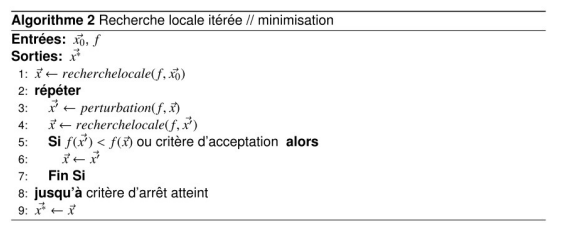
\includegraphics[width=0.9\textwidth]{algo.png}
    \caption{Algorithme pseudo-code Recherche Locale Itérée}
    \label{fig:mon_image}
\end{figure}
Ce pseudo-code donne un aperçu de la structure générale de l’algorithme de la recherche locale itérée et peut être adapté selon les besoins spécifiques du problème du sac à dos.
\end{frame}

\begin{frame}{Code Python}
	 \begin{block}{Codes}
   		Illustration de l'implementation sur Python
\end{block}
\end{frame}
% Section 4: Étude Comparative
\section{Étude Comparative}
\begin{frame}{Résultats obtenue: 1ere execution}
   \begin{figure}[h]
    \centering
    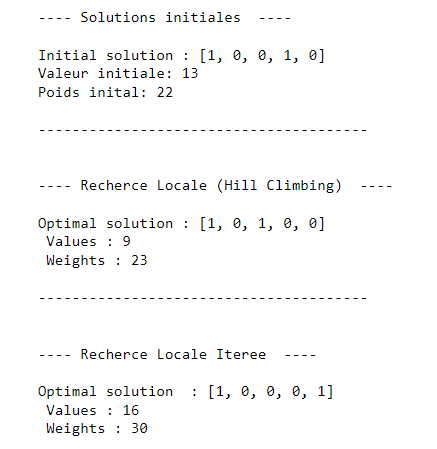
\includegraphics[width=0.5\textwidth]{solution1.png}
    \caption{Algorithme pseudo-code Recherche Locale Itérée}
    \label{fig:mon_image}
\end{figure}
\end{frame}
\begin{frame}{Résultats obtenue  : Sur 10 instances nous obtenons}
   \begin{figure}[h]
    \centering
    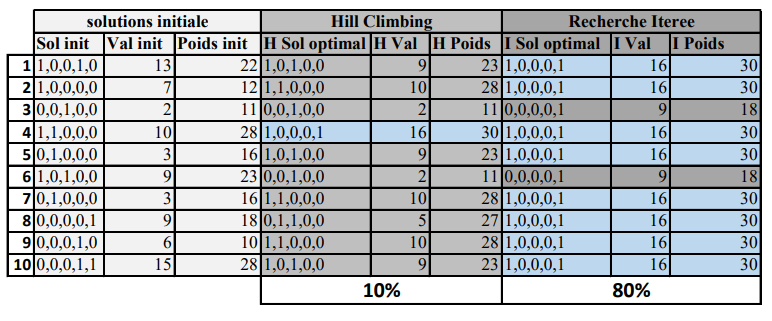
\includegraphics[width=0.9\textwidth]{stat.png}
    \caption{Algorithme pseudo-code Recherche Locale Itérée}
    \label{fig:mon_image}
\end{figure}
\end{frame}

% Section 6: Conclusion
\section{Conclusion}
\begin{frame}{Conclusion}
    \begin{itemize}
\item Nous avons exploré la méthode de recherche locale itérée pour résoudre le problème du sac à dos.
\item Examen approfondi de la méthode de recherche locale itérée, de ses avantages et inconvénients, comparaison avec le Hill Climbing.
\item Discussion sur l'implémentation pratique de la méthode, présentation d'un pseudo-code.
\item La recherche locale itérée représente un outil puissant pour résoudre des problèmes complexes, offrant un équilibre entre efficacité, simplicité et adaptabilité.
\end{itemize}
\end{frame}

\begin{frame}
\begin{minipage}{0.48\textwidth}
\centering

\includegraphics[width=\textwidth]{merci2.png}
\end{minipage}\hfill
\begin{minipage}{0.48\textwidth}
\centering

\includegraphics[width=\textwidth]{question.png}
\end{minipage}
\end{frame}
\end{document}